%\documentclass{cumcmthesis}
\documentclass[withoutpreface,bwprint]{cumcmthesis} %去掉封面与编号页,电子版提交的时候使用。



\usepackage{url}   % 网页链接
\usepackage{booktabs}
\usepackage{array}
\usepackage{subcaption} % 子标题
\usepackage{amsmath}
\usepackage{amssymb}
\title{基于最小二乘原理的主客观组合权重法及结构方程评价模型}
\tihao{A}
\baominghao{}
\schoolname{东北大学秦皇岛分校}
\membera{ }
\memberb{ }
\memberc{ }
\supervisor{ }
\yearinput{2022}
\monthinput{07}
\dayinput{08}

\begin{document}
 \maketitle
 
 
 \begin{abstract}
2022年北京冬奥会于2月20日顺利闭幕。奥运会是一项集体育,政治,经济,文化于一身的超级国际盛会,对于举办国的影响是长久而深远的。
然而在新冠肺炎疫情的全球背景下,奥运会对于中国的GDP,旅游,投资在短期内也许并不那么显而易见,而突破了地域,种族,性别的文化却可以顺着网线到达千家万户。文化是国家发展、民族进步最深远,最持久的力量。奥运会作为文化输出的窗口,其影响力不亚于对政治,经济的影响。因此,本文探究冬奥会的文化影响力,并假设北京冬奥会具有一定的文化影响力,这种文化影响力能都让一定比例的人参加到冰雪运动中来,进而探究我国是否实现了“带动三亿人参与冰雪运动”的目标。



\textbf{模型一(最小二乘原理的主客观组合权重法)}:通过收集到的百度指数“冰墩墩”、“北京奥运会”,谷歌趋势“北京奥运会”搜索指数数据进行定性分析比较,发现冬奥通过自身的文化魅力,吸引了大众的关注,因此研究北京冬奥会的文化影响力是可行的。首先对近四年冬奥会数据使用\textbf{层次分析法}进行主观赋权,使用\textbf{Topsis熵权法}进行客观赋权,然后通过\textbf{最小二乘原理}对权重进行组合优化,并计算得分。最后得出结论:\textbf{北京冬奥会是冬奥会史上文化影响力最大的一届,其影响力相当于平昌冬奥会的10倍。}

\textbf{模型二(结构方程模型)}:首先在模型一的基础上,选取“关注程度”、“举办满意度”、“北京冬奥会影响力”三个指标,设置问卷调查大众对三个指标的评价,通过收集到的问卷数据建立\textbf{结构方程模型}。然后假设北京冬奥会存在一个文化影响因子,通过结构方程模型个指标间的相关性计算得出文化影响因子的值为$0.399$。最后得出结论:\textbf{北京冬奥会的举办将会带动约5.6亿人参与冰雪运动,中国能够实现了“带动三亿人参与冰雪运动”的目标。}
 







\keywords{层次分析法\quad  Topsis熵权法\quad   最小二乘原理主客观组合权重法\quad  结构方程模型}
\end{abstract}

%目录  2019 明确不要目录,我觉得这个规定太好了
%\tableofcontents

%\newpage

\section{问题重述}
\subsection{问题背景}
2022年北京冬奥会于2月20日顺利闭幕。奥运会作为一项集体育,政治,经济,文化于一身的超级国际盛会,对于举办国的影响是长久而深远的。
然而在新冠肺炎疫情的全球背景下,奥运会对于中国的GDP,旅游,投资在短期内也许并不那么显而易见,而突破了地域,种族,性别的文化却可以顺着网线到达千家万户。文化是国家发展、民族进步最深远,最持久的力量。奥运会作为文化输出的窗口,其影响力不亚于对政治,经济的影响。因此,探究2022年冬奥会的文化影响力具有重要意义。
\subsection{指标选择}
	针对第一问,为了探究奥运会的文化影响力,选取了百度指数“冰墩墩”、“北京冬奥会”,谷歌趋势“北京冬奥会”的搜索指数数据以及最近四年的冬奥会数据作为研究对象。
	
	针对第二问,为了估算参与冰雪运动的总人数,发放了北京奥运会影响力调查问卷,见附录一。
	
\subsection{具体问题}

\begin{enumerate}
	\item 根据百度指数“冰墩墩”、“北京奥运会”,谷歌趋势“北京奥运会”搜索指数数据,定性分析2022冬奥会文化影响力;
	\item 根据最近四年冬奥会数据,建立数学模型,定量的分析2022冬奥会文化影响力
	\item 根据模型一结果和问卷数据,建立数学模型,估算2015申奥成功至今全民参与冰雪运动的总人数。
\end{enumerate}
	
\clearpage

\section{问题分析}
   评判奥运会的影响力,首先要确定合适的评判标准。奥运会的影响主要体现在GDP,旅游,投资等方面,然而在新冠肺炎全球大背景下,奥运会对北京和张家口短期内的影响并不显著,甚至是负增长。因此选取了文化作为评判2022北京冬奥会的标准。奥运文化作为一种深入人心的影响力,能够带动更多人参与到冰雪运动中来,假定申奥成功以后,奥运会每年具有一定的文化影响力,而这种文化影响力,每年能够带动一定比例的群众参与到冰雪运动中来,那么可以使用文化影响力来探究奥运会的开幕能否带动3亿人参与到冰雪运动中来。本论文的研究思路如下:\begin{figure}[H]
   	\centering
   	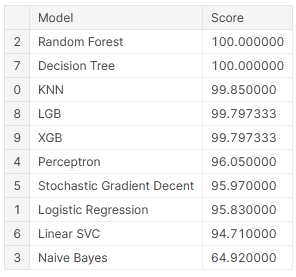
\includegraphics[scale=0.11,angle=0]{10.png}
   	\caption{论文思路图}
   	\label{10}
   \end{figure}
   
		
\section{模型假设}
\begin{enumerate}
	\item 假设疫情对奥运文化的传播没有影响
	\item 假设百度指数和谷歌趋势和中国及世界关注奥运会的趋势是一样的;
	\item 假设奥运会具有一定的文化影响力,而这种影响力能够让一定比例的群众参加冰雪运动。
\end{enumerate}

\clearpage
\section{符号说明}
\begin{table}[h]
	\begin{center}
		\begin{tabular}{p{240pt}p{250pt}}
			\toprule
			符号    & 含义  \\
			\midrule
			$A,B,\dots$     &   矩阵 \\
			$A^T$  &  矩阵A的装置 \\
			$A^{-1}$  &  矩阵A的逆 \\
			$a_{ij}$ & 矩阵A中的第i行第j列的元素   \\
			$\mu$  &  样本平均值 \\	
			$\sigma$  &  样本标准差 \\	
			$\sum$  &  求和符号 \\
			$CI$  & 一致性指标 \\
			$CR$  & 一致性比例\\
			$max\{\},min\{\}$  & 求最大值和最小值 \\	
		
			$\operatorname{diag}\left[\lambda_{1},\lambda_{2},\dots,\lambda_{n}\right]$  & 对角线元素为$\lambda_{1},\lambda_{2},\dots,\lambda_{n}$的对角矩阵\\
				$\frac{\partial L}{\partial \lambda}$  &  求L关于$\lambda$d的偏导数    \\	
			$ \left[\begin{array}{cc}\mathrm{A} & \mathrm{e} \\ \mathrm{e}^{\mathrm{T}} & 0\end{array}\right]$  &  分块矩阵 \\
		
			
			\bottomrule
		\end{tabular}
	\end{center}
\end{table}

\section{问题一模型的建立与求解}
\subsection{使用对比分析法定性评价北京冬奥会的文化影响力}
北京冬奥会于2022年2月4日开幕,举国沸腾。根据奥运会举办期间百度“冰墩墩”“北京奥运会”搜索指数及咨询关注,绘制折线图如图:
\begin{figure}[H]
	\centering
	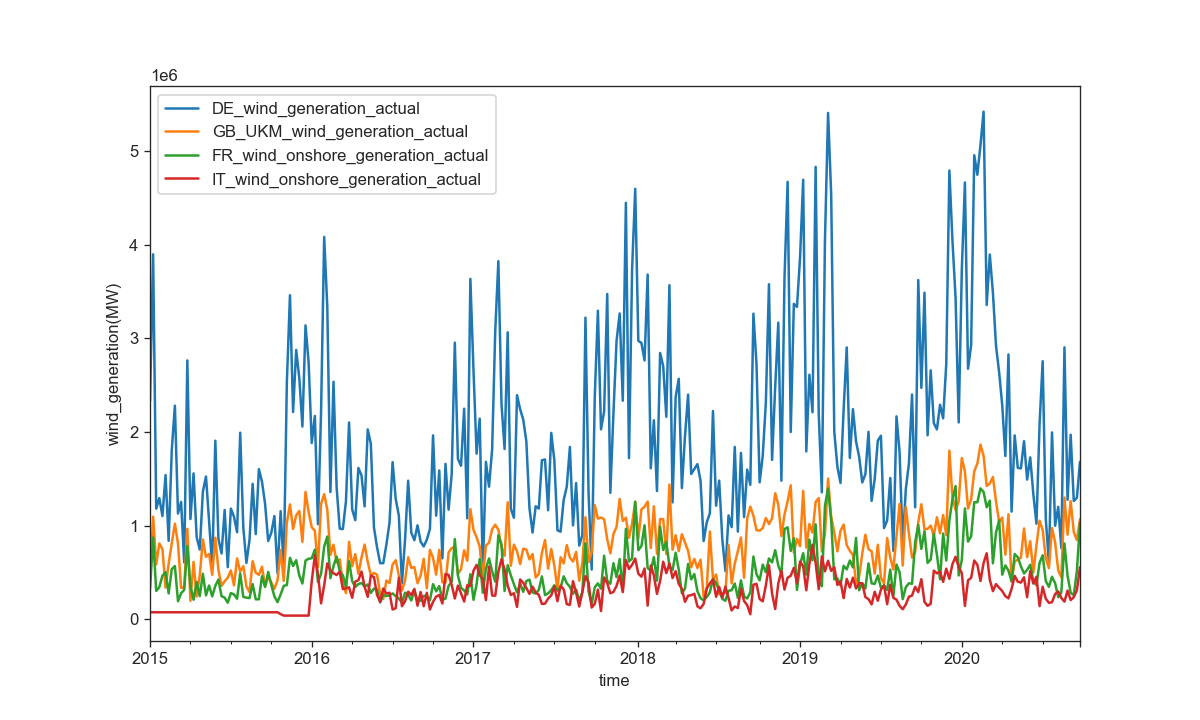
\includegraphics[scale=0.25,angle=0]{2.png}
	\caption{冬奥会期间民众关注程度}
	\label{2}
\end{figure}
结果显示,民众对北京冬奥会的关注热情一直高涨,在奥运会举办期间达到高潮。而“北京奥运会”搜索指数,“冰墩墩”资讯关注度,“冰墩墩”搜索指数也在奥运会举办期间达到高潮。仅2021年10月29日到2022年03月10日,“北京冬奥会”资讯关注度就达到3.01亿次,“北京奥运会”搜索指数达6000万次,“冰墩墩”资讯关注度,“冰墩墩”搜索指数分别达0.93亿次,0.15亿次。说明北京冬奥会在国内引起了热烈反响。

根据谷歌趋势对四个奥运会的搜索趋势数据,绘制如下图形:
\begin{figure}[H]
	\centering
	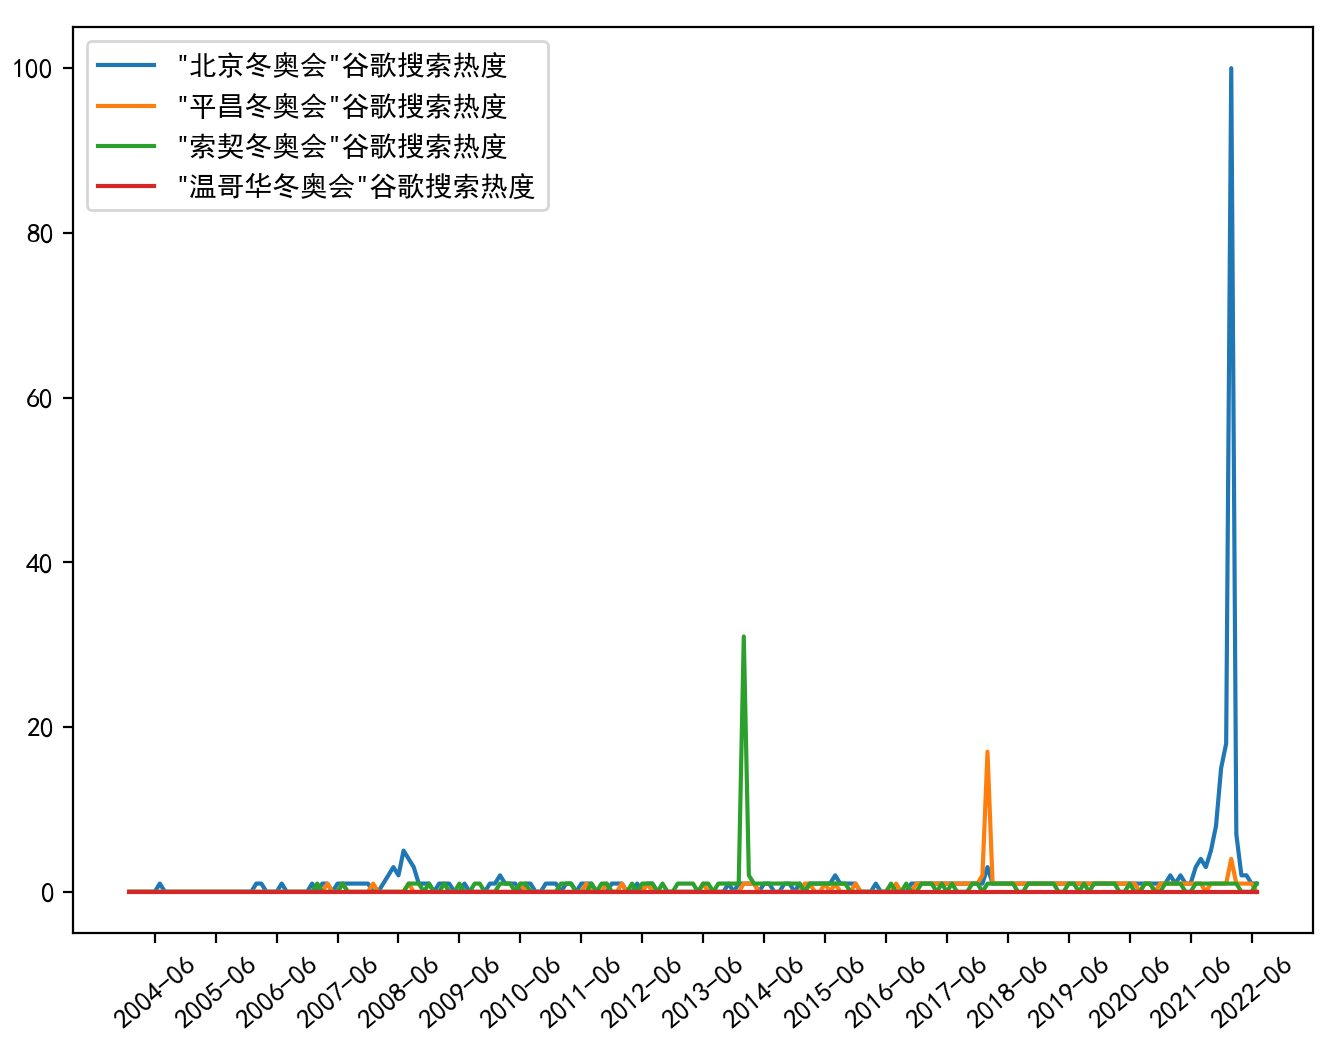
\includegraphics[scale=0.25,angle=0]{5.png}
	\caption{冬奥会期间民众关注程度}
	\label{5}
\end{figure}
结果显示,全球对北京冬奥会的关注程度远远超过了往届冬奥会,说明北京冬奥会在国外也引起了热烈反响。

从以上的结果可以看出,北京冬奥会无论在国内还是在国外,其关注程度都远远超过了往届冬奥会。

\subsection{基于最小二乘原理的主客观组合权重法评价北京冬奥会的影响力}
	考虑到数据的有效性和可获取性,初步选取了以下指标,数据来源于百度百科,百度指数及谷歌趋势。
\begin{figure}[H]
	\centering
	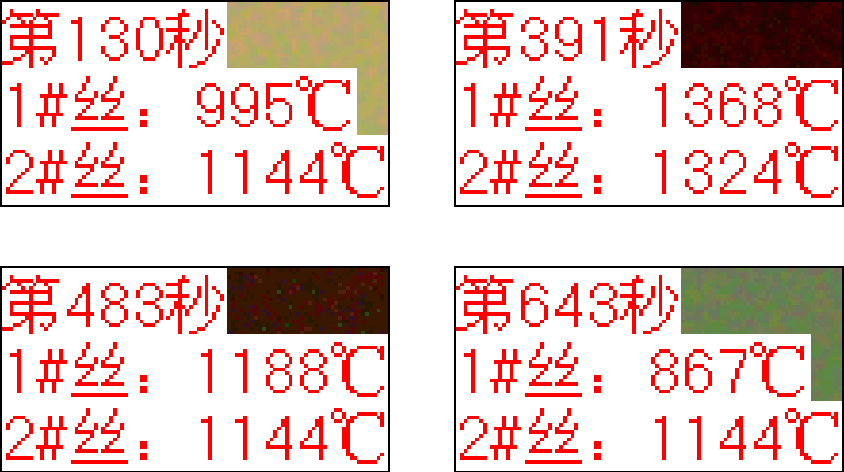
\includegraphics[scale=0.5,angle=0]{1.png}
	\caption{初步选取的指标数据}
	\label{1}
\end{figure}
其中预计观看人数为根据新闻媒体报道采集的数据,单位为亿,百度资讯指数及搜索指数为奥运会举办前后共3年搜索指数及趋势的平均值,谷歌趋势则是四个奥运会搜索热度最大值的相对百分比,令
\[A=\begin{bmatrix}%长中括号包裹的矩阵
109 & 91 & 2892 & 20 &  341238& 58457 & 100\\
102 & 92 & 2922 & 6 & 34249 & 2116 & 18\\
98 &  88& 2873 & 14 & 10433 & 1288 & 31\\
86 & 85 &  2750& 6 & 6143 & 168 &1
\end{bmatrix}
\]



首先对数据进行KMO检验,以确定是否有降维的必要。由于样本数据太少继续收集了往前三年的数据以进行KMO检验,KMO检验结果的平均值为0.30,说明数据之间具有一定的独立性,能够提供特定的信息,不必进行进一步的数据降维操作。
	
	
\subsubsection{主观赋权——层次分析法}
层次分析法是一种应用网络系统理论和多目标综合评价方法,提出的一种层次权重决策分析方法。层次分析法将问题分解成有关因素,并根据这些因素之间的关系分类形成多层次的结构模型。在此基础上进行定量定性分析,利用较少的定量信息,将决策的思维过程数学化。以此来解决一些相互关联相互制约的,众多因素构成的复杂系统的决策问题。

层次分析法一般包括建立层次模型,构造判断矩阵,层次排序和一致性检验等步骤。首先构造层次模型,模型根据目标层–准则层–方案层构建层次模型图如下:
\begin{figure}[H]
	\centering
	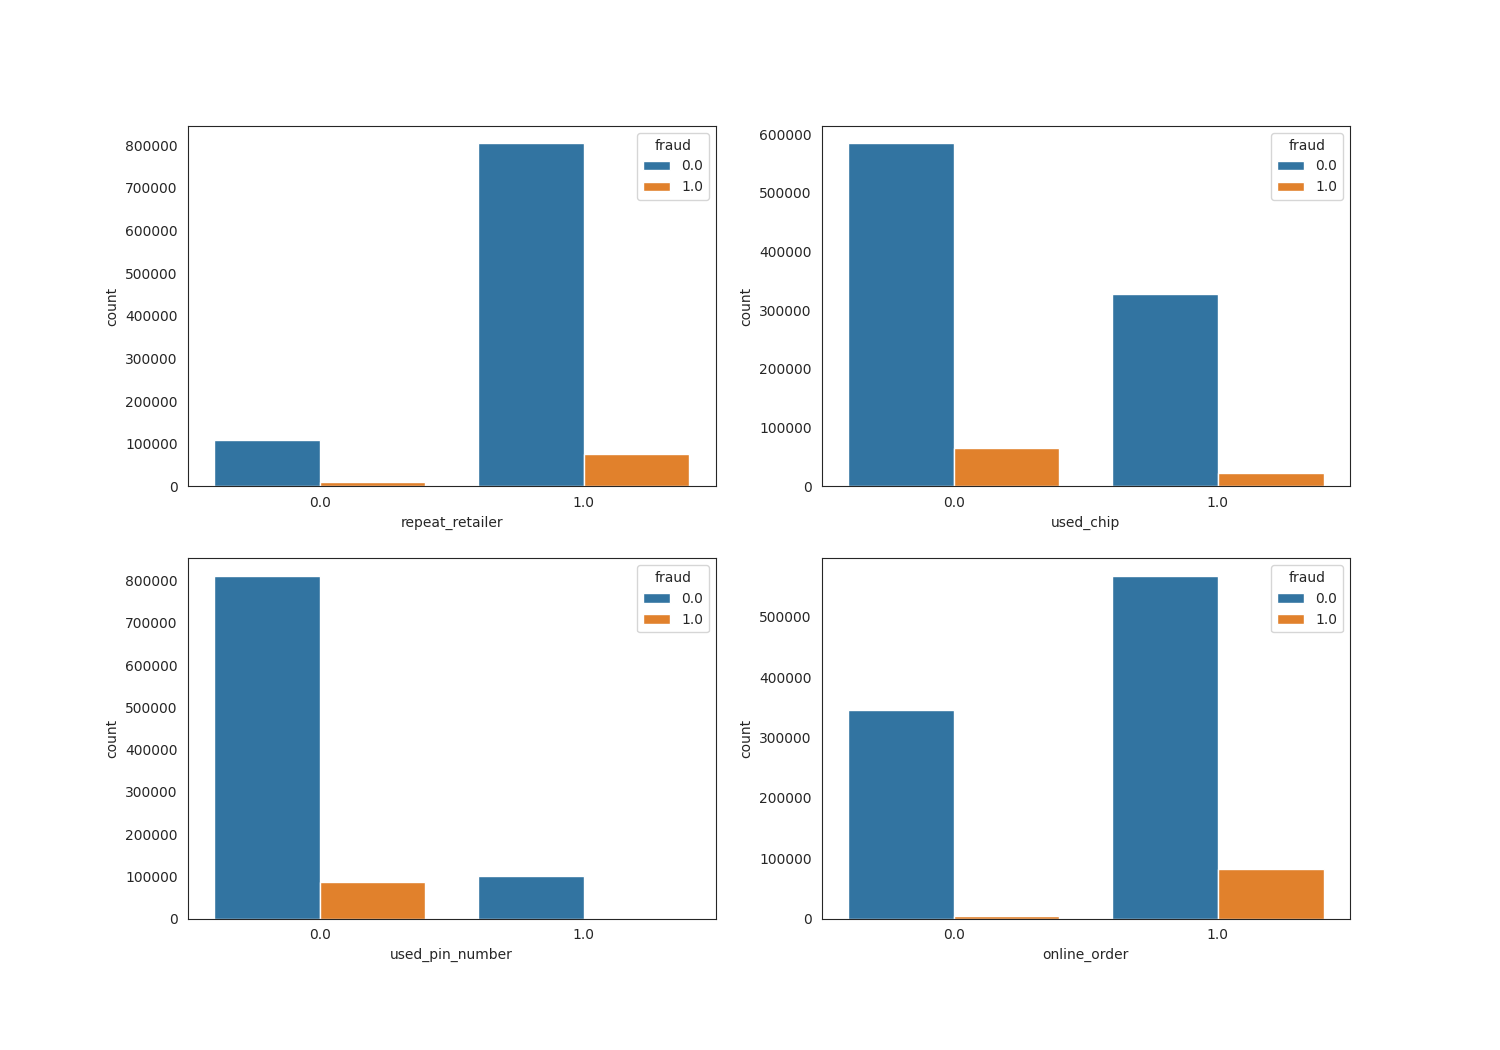
\includegraphics[scale=0.5,angle=0]{6.png}
	\caption{层次模型图}
	\label{6}
\end{figure}
判断矩阵是衡量每两个指标之间重要性的矩阵,矩阵上每个元素对应了该行该列对应指标的间的相对重要程度。现对在层次结构图中的第二层构造判断矩阵,在构造判断矩阵时,为了避免定性的不准确性,使用一致矩阵法构造判断矩阵。根据Saaty的1-9标度方法构造出的判断矩阵如下:
\[J=\begin{bmatrix}%长中括号包裹的矩阵
1 & 5 & 5 & 2 &  2& 4 & 5\\
\frac{1}{5} & 1 & 1 & \frac{1}{4} & \frac{1}{5} & 2 & 1\\
\frac{1}{5} &  1& 1 & 1& 1 & 2 & 3\\
\frac{1}{2} & 4 &  1& 1 & 1 & 3 &4\\
\frac{1}{2} & 5 & 1 & 1 & 1 & 3 & 4\\
\frac{1}{4} &  \frac{1}{2}& \frac{1}{2} & \frac{1}{3}& \frac{1}{3} & 1 & 3\\
\frac{1}{5} & 1 &  \frac{1}{3}& \frac{1}{4} & \frac{1}{4} & \frac{1}{3} &1\\
\end{bmatrix}
\]

为了进行一致性检验,首先建立一致性指标。根据判断矩阵,可以求得其最大特征值$\lambda _{max}$ = 	7.435,则一致性计算指标为:
$$CI=\frac{\lambda _{max}-n}{n-1}$$

在一致性指标的基础上计算一致性比例,通过查表可以得$n=7$时,平均随机一致性指标$RI = 1.36$,则一致性比例为
$$CR=\frac{CI}{RI},$$求得$CR=0.053<0.1$,通过一致性检验,认为判断矩阵的不一致程度在容许范围之内,故可对其进行归一化采用特征值法求取权重得:$$U=\left[\begin{array}{lllllll}
0.336 & 0.07 & 0.119 & 0.176 & 0.186 & 0.068 & 0.045
\end{array}\right]
$$	
\subsubsection{客观赋权——Topsis熵权法}
基于熵权法对Topsis模型是一种常用的综合评价方法,该方法能充分利用原始数据信息,在有限方案中的找出最优方案和最劣方案,并计算各评价对象与最优方案和最劣方案之间的距离,根据各评价对象与最优方案的相对接近程度来判断评价对象的优劣。其结果能客观反映各个评价方案之间的差距。

Topsis熵权法需要所有的指标都为极大型指标,由于数据中的指标均是极大型指标,因此不必再进行指标正向化。 对数据进行标准化,标准化公式为:$$x_{ij} = \frac {x_{ij}-\mu}{\sigma},$$其中 $ \mu $ 和$ \sigma $ 分别是样本数据的均值和标准差。
标准化发现数据中含有负值,为了将数据映射到$[0-1]$,故对数据进行归一化,归一化公式为:$$\tilde{z}_{i j}=\frac{x_{i j}-\min \left\{x_{1 j}, x_{2 j}, \cdots, x_{n j}\right\}}{\max \left\{x_{1 j}, x_{2 j}, \cdots, x_{n j}\right\}-\min \left\{x_{1 j}, x_{2 j}, \cdots, x_{n j}\right\}},$$
归一化的数据消除了量纲以及数据差异性的影响,并且使数据在0和1的范围内。使用归一化后的数据计算概率矩阵,计算公式为:$$p_{i j}=\frac{\tilde{z}_{i j}}{\sum_{i=1}^{n} \tilde{z}_{i j}}$$
概率矩阵的每一项都是一个表示概率的非负实数,通过概率矩阵计算5个指标的信息熵:$$e_{j}=-\frac{1}{\ln n} \sum_{i=1}^{n} p_{i j} \ln \left(p_{i j}\right)(j=1,2, \cdots, 5)$$其中,如果$p_{ij}=0$,则令$ln(p_{ij})=0$,计算结果为:$$e=\left[\begin{array}{lllllll}
0.258 & 0.261 & 0.284 & 0.179 & 0.126 & 0.119 & 0.183
\end{array}\right]
$$
使用公式$d_j=1-e_j$计算信息效用值得$$d=\left[\begin{array}{lllllll}
0.258 & 0.261 & 0.284 & 0.179 & 0.126 & 0.119 & 0.183
\end{array}\right]
$$
在信息效用值得基础上计算熵权,使用
$$V_{j}=
\frac{d_{j}} { \sum_{j=1}^{5} d_{j}}(j=1,2, \cdots, 5)$$计算得到客观赋权的权重值$$V=\left[\begin{array}{lllllll}
0.133 & 0.132 & 0.128 & 0.147 & 0.156 & 0.158 & 0.146
\end{array}\right].$$
\subsubsection{基于最小二乘原理的主客观组合权重法}
最小二乘法是通过最小化误差的平方和确定最佳参数的方法,从而使得这些求得的数据与实际数据之间误差的平方和为最小。无论是主观赋权法还是客观赋权法,都有一定的弊端。本文使用最小二乘法对两种赋权法进行优化组合,假设优化后的权重为$$\mathrm{W}=\left[\mathrm{w}_{1}, \mathrm{w}_{2}, \mathrm{w}_{3},\mathrm{w}_{4},\mathrm{w}_{\mathrm{5}}\right]^{\mathrm{T}},$$则第$i$个评价对象的评价值为
$$\mathrm{f}_{\mathrm{i}}=\sum_{\mathrm{i}=1}^{\mathrm{m}} \mathrm{w}_{\mathrm{j}} \mathrm{Z}_{\mathrm{ij}},(\mathrm{i}=1,2, 3 \dots \mathrm{m}),$$
对于W,希望与主客观的评价值越小越好,因此
$$\begin{array}{c}
	\min \mathrm{H}(\mathrm{w})=\sum_{i=1}^{\mathrm{n}} \sum_{i=1}^{\mathrm{m}}\left\{\left[\left(\mathrm{u}_{\mathrm{j}}-\mathrm{w}_{\mathrm{j}}\right) \mathrm{z}_{\mathrm{ij}}\right]^{2}+\left[\left(\mathrm{v}_{\mathrm{j}}-\mathrm{w}_{\mathrm{j}}\right) \mathrm{z}_{\mathrm{i}}\right]^{2}\right\} \\
	\sum_{\mathrm{j}=1}^{\mathrm{m}} \mathrm{w}_{\mathrm{j}}=1, \mathrm{w}_{\mathrm{j}} \geqslant 0(\mathrm{j}=1,2,3,4,5)
\end{array},$$
为了求解此模型,作Langrange函数
$$L=\sum_{i=1}^{n} \sum_{j=1}^{m}\left\{\left[\left(u_{j}-w_{j}\right) z_{i j}\right]^{2}+\left[\left(v_{j}-w_{j}\right) z_{i j}\right]^{2}\right\}+4 \lambda\left(\sum_{j=1}^{m} w_{j}-1\right),$$对$w_i$求偏导数得
$$\frac{\partial \mathrm{L}}{\partial \mathrm{w}_{\mathrm{j}}}=-\sum_{\mathrm{i}=1}^{\mathrm{n}} 2\left(\mathrm{u}_{\mathrm{j}}+\mathrm{v}_{\mathrm{j}}-2 \mathrm{w}_{\mathrm{j}}\right) \mathrm{z}_{\mathrm{ij}}^{2}+4 \lambda=0 \quad(\mathrm{j}=1,2, \cdots, \mathrm{m}),$$
对$\lambda$求偏导数得
$$\frac{\partial L}{\partial \lambda}=4\left(\sum_{i=1}^{m} w_{j}-1\right)=0,$$
用矩阵表示为 $$ \left[\begin{array}{cc}\mathrm{A} & \mathrm{e} \\ \mathrm{e}^{\mathrm{T}} & 0\end{array}\right] \cdot\left[\begin{array}{c}\mathrm{W} \\ \lambda\end{array}\right]=\left[\begin{array}{l}\mathrm{B} \\ 1\end{array}\right] ,$$
\text{其中  $A=\operatorname{diag}\left[\sum_{i=1}^{n} z_{i 1}^{2}, \sum_{i=1}^{n} z_{i 2}^{2}, \cdots, \sum_{i=1}^{n} z_{i m}^{2}\right] $ 是一个$  m \times m $ 的对角阵,} $e=[1,1, \cdots, 1]^{T} $、$ W $、
$ B$  均为 $ m \times 1 $ 维向量。其中$$B=\left[\sum_{i=1}^{n} \frac{1}{2}\left(u_{1}+v_{1}\right) z_{i 1}^{2}, \sum_{i=1}^{n} \frac{1}{2}\left(u_{2}+v_{2}\right) z_{i 2}^{2}, \cdots, \sum_{i=1}^{n} \frac{1}{2}\left(u_{m}+v_{m}\right) z_{i m}^{2}\right]^{T},$$
解上面的矩阵方程,得
$$\mathrm{W}=\mathrm{A}^{-1} \cdot\left[\mathrm{B}+\frac{1-\mathrm{e}^{\mathrm{T}} \mathrm{A}^{-1}\mathrm{~B}}{\mathrm{e}^{\mathrm{T}} \mathrm{A}^{-1} \mathrm{e}} \cdot \mathrm{e}\right],$$
根据最小二乘原理组合主客观权重的公式,得
$$W=\left[\begin{array}{lllllll}
0.229 & 0.096 & 0.119 & 0.154 & 0.211 & 0.103 & 0.089
\end{array}\right]
.$$
使用最终得到的权重,可以求得四个冬奥会的得分
$$S=AW^T,$$
对S中的数据进行归一化,归一化公式为$$s_{j}=\frac{s_{j}}{\sum_{i=1}^{m} s_i},j=1,2,3,4.$$
得到最终结果$$S=\left[\begin{array}{llll}
84.82 & 8.81 & 3.79 & 2.57
\end{array}\right]
.$$

从计算得出的数据中可以看出,2022北京冬奥会的评分几乎是2018平昌冬奥会的评分的十倍,而索契冬奥会和温哥华冬奥会的评分则比较低,北京奥运会与以往三次冬奥会相比具有极高的评分。近几年互联网的迅猛发展,为全球人民提供了了解更多资讯的平台,也为各国文化传播提供了一个传播更迅速的平台,因此从互联网资讯指数以及搜索指数中可以看出一件事物的受欢迎程度和影响力。从2022北京冬奥会远超前几次冬奥会的互联网资讯指数和搜索指数,以及极高的评分中可以看出,2022北京冬奥会受欢迎程度极高,他对世界各国人民的文化影响力是巨大的。

\section{模型二——结构方程模型}
结构方程模型是一种社会学方法,基于变量的协方差矩阵来来分析变量之间的关系,又称协方差结构分析。
有很多概念是无法直接准确测量的,这种变量称为潜在变量,需要用一些外显指标(观测变量)来间接反映这些变量的关系。传统的统计方法是无法处理潜在变量的,但是结构方程模型可以很好的处理观测变量与潜变量之间的关系。
结构方程模型包括测量模型和结构模型,测量模型指的是观测变量与潜在变量之间的关系,而结构模型则分析潜在变量之间的关系。
本文设置3个外生潜在变量和1个内生潜在变量,具体潜在变量与对应的观测变量的设置如下:
\begin{figure}[H]
	\centering
	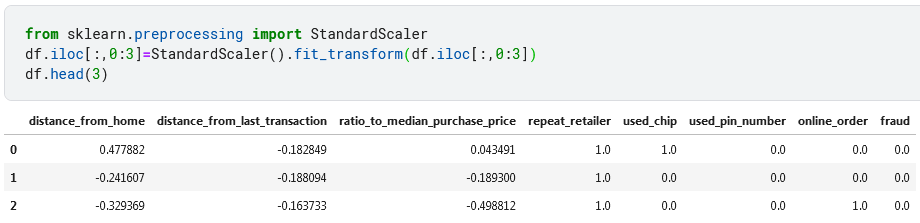
\includegraphics[scale=0.4,angle=0]{7.png}
	\caption{观测指标的设置}
	\label{7}
\end{figure}
为此我们收集了67份数据,数据显示,参加过冰雪运动的比例为38.63\%,按此计算,截止到2022年7月8日,保守估计将会有14$ \times $ 38.63\% =5.4亿人参加到冰雪运动中来,但这并不能很好的体现东奥文化对参与冰雪运动的促进作用,因此考虑建立结构方程模型进一步对参与冰雪运动的人数进行量化。
\begin{figure}[H]
	\centering
	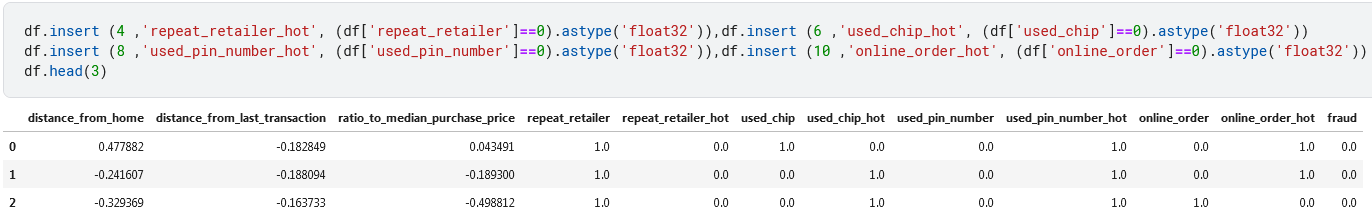
\includegraphics[scale=0.9,angle=0]{8.png}
	\caption{问卷中参与冰雪运动比例}
	\label{8}
\end{figure}
结构方程模型包括测量模型与结构模型,其中测量模型可以得出观测指标与潜在变量之间的关系;结构模型可以得出潜在变量与潜在变量之间的关系。结构方程模型可以以下三个公式表示:
\begin{align}
	\eta=\beta \eta+\Gamma \xi+\zeta \\
	y=\Lambda_{\eta}+\varepsilon \\
	x=\Lambda_{\eta}+\sigma
\end{align}
方程(3)是结构模型,它通过Γ系数矩阵以及误差向量ζ把潜在变量联系起来。方程(4)和方程(5)是测量模型,通过这两套线性方程连接观测变量与对应潜在变量η和ξ。根据选择的指标和公式可得测量方程为:

\begin{center}
$
\left(\begin{array}{c}
	\text { ate1 } \\
	\text { ate2 }  \\
	\text { ate3 }  \\
	\text { ate4 }  \\
	\text { sat1 } \\
	\text { sat2 } \\
	\text { sat3 } \\
	\text { sat4 } \\
	\text { afe1 } \\
	\text { afe2 }  \\
	\text { afe3 }  \\
	\text { afe4 }  
\end{array}\right)=\left(\begin{array}{ccc}
	\lambda_{1} & 0 & 0 \\
	\lambda_{2} & 0 & 0 \\
	\lambda_{3} & 0 & 0 \\
	\lambda_{4} & 0 & 0 \\
	0 & \lambda_{5} & 0 \\
	0 & \lambda_{6} & 0 \\
	0 & \lambda_{7} & 0 \\
	0 & \lambda_{8} & 0 \\
	0 & 0 & \lambda_{9} \\
	0 & 0 & \lambda_{10} \\
	0 & 0 & \lambda_{11} \\
	0 & 0 & \lambda_{12}
\end{array}\right)\left(\begin{array}{c}
	\xi_{1} \\
	\xi_{2} \\
	\xi_{3}
\end{array}\right)+\left(\begin{array}{c}
	\sigma_{1} \\
	\sigma_{2} \\
	\sigma_{3} \\
	\sigma_{4} \\
	\sigma_{5} \\
	\sigma_{6} \\
	\sigma_{7} \\
	\sigma_{8} \\
	\sigma_{9} \\
	\sigma_{10} \\
	\sigma_{11} \\
	 \sigma_{12} 
\end{array}\right) 
,$

$
\left(\begin{array}{c}
	\text { par1 }  \\
	\text { par2 }  \\
	\text { par3 }  \\
	\text { par4 }  \\
	\text { par5 }  \\
	\text { par6 } 
\end{array}\right)=\left(\begin{array}{c}
	\lambda_{13} \\
	\lambda_{14} \\
	\lambda_{15} \\
	\lambda_{16} \\
	\lambda_{17} \\
	\lambda_{18}
\end{array}\right)\left(\begin{array}{c}
	\eta_{1}
\end{array}\right)+\left(\begin{array}{c}
	\varepsilon_{1} \\
	\varepsilon_{2} \\
	\varepsilon_{3} \\
	\varepsilon_{4} \\
	\varepsilon_{5} \\
	\varepsilon_{6}
\end{array}\right)
.$

\end{center}
结构方程为
\begin{center}
$
\eta_{1}=\begin{array}{c}
	\beta
\end{array}\begin{array}{c}
	\eta_{1} \\
	
\end{array}+\left(\begin{array}{ccccc}
	\gamma_{1} & \gamma_{2} & \gamma_{3} & \gamma_{4} & \gamma_{5}
\end{array}\right)\left(\begin{array}{c}
	\xi_{1} \\
	\xi_{2} \\
	\xi_{3} \\
	\xi_{4} \\
	\xi_{5}
\end{array}\right)+\begin{array}{c}
	\zeta_{1}
\end{array}
,$
\end{center}
其中, 第一个方程是外生潜在变量的测量方程,  $\lambda_{1}, \lambda_{2}, \cdots, \lambda_{12} $ 是外生潜在变量的观测指标,  $\xi_{1}, \xi_{2} \cdots \xi_{5}  $是外生潜在变量的因子载荷, $ \sigma_{1}, \sigma_{2} \cdots \sigma_{1}$  是 $ \xi_{1}, \xi_{2} \cdots \xi_{5}  $的观测指标的 测量误差; 第二个方程是内生潜在变量的测量方程, $ \lambda_{13}, \lambda_{14} \cdots \lambda_{18} $ 是内生潜在变量的测量 指标, $ \eta_{1} $ 是内生潜在变量的因子载荷,$  \varepsilon_{1}, \varepsilon_{2} \cdots \varepsilon_{6} $ 是 $ \eta_{1}  $的观测指标的测量误差。 第三个方程 是潜在变量之间的结构方程,  $ \beta  $ 是 $  \mathrm{B}  $ 的回归系数矩阵; $ \left(\begin{array}{lllll}\gamma_{1} & \gamma_{2} & \gamma_{3} & \gamma_{4} & \gamma_{5} \end{array}\right)$  是 $ \Gamma$  的回归系数矩阵;  $\zeta_{1}, \zeta_{2}  $是  $\eta_{1}$ 的残差。

对收集到的问卷进行信度检验和效度检验。根据AMOS的结果显示,$Chonbach.\alpha$的值为$0.841$,数据具有很高的可信度,通过信度检验;KMO的值为0.796,数据通过效度检验。使用AMOS对模型进行求解并绘制图形如下:
\begin{figure}[H]
	\centering
	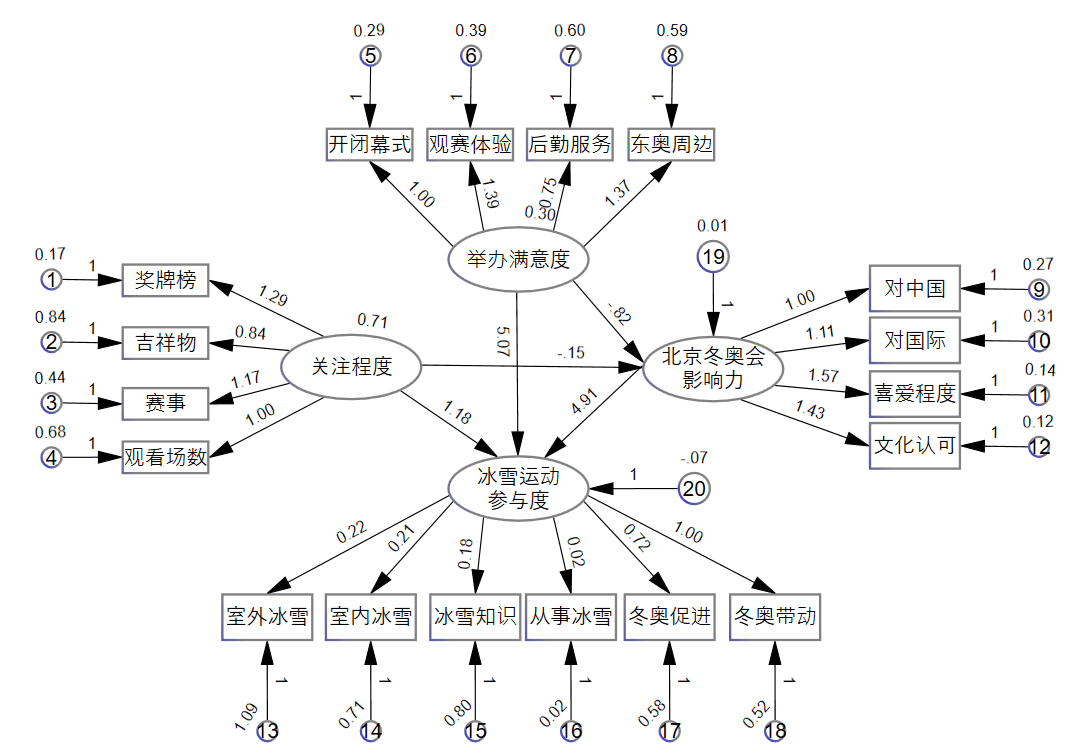
\includegraphics[scale=0.5,angle=0]{9.png}
	\caption{结构方程模型结果}
	\label{9}
\end{figure}

模型结果显示,冰雪运动的参与度与被访者的关注程度,举办满意度,北京冬奥会的影响力均成正相关。为了具体量化冰雪参与度与其他潜在变量的关系,定义文化影响力因子$\delta$,假设文化影响力因子与关注程度,举办满意度,北京冬奥会影响力的相关性为$\rho_1,\rho_2,\rho_3$。对相关性进行归一化,公式为$$\frac{\rho_1}{\rho_1+\rho_2+\rho_3},$$以此类推关注程度,举办满意度,北京冬奥会影响力的计算方法,最后根据67份问卷数据计算最终的文化影响力因子$$\delta=0.399$$,意味着冬奥会将会带动全国39.9\%的人参与到冰雪运动中来,即$14 \times 39.9\%=5.6$亿人参与到冰雪运动中来,因此中国实现了带动三亿人参与冰雪运动的目标。

\section{模型评价与改进}
\subsection{模型总结}
针对问题一,通过定性分析和定量计算,分析了北京冬奥是所有冬奥会中最具文化影响力的一届。针对问题二,假设北京奥运会有一定的文化影响力,这种文化影响力能够带动一定比例的人参加冰雪运动,通过计算。冬奥会的开展大约能够使5.6亿人参与到冰雪运动中来,因此中国实现了带动3亿人参与冰雪运动中来的目标。
\subsection{优点}
\begin{enumerate}
	\item  \textbf{定性分析与定量计算结合}。针对问题一,先对收集到的数据进行数据分析,定性的评价北京冬奥会的影响力;针对问题二,先使用问卷中参加冰雪运动比例估算全国参与冰雪运动的人数,在建立结构方程模型,定量的全国参与冰雪运动的人数。
	\item \textbf{主观与客观结合}。模型一中,先使用层次分析法进行主观赋权,再使用Topsis熵权法进行赋值,最后使用最小二乘原理对主客观赋值进行组合优化。
	\item \textbf{原理简单,便于操作}。结构方程模型通过可观测变量反映潜在指标,容易理解,且建模方法简单,使用方便。
	\item \textbf{对数据要求低,功能强大}。可以同时处理多个变量,对于数据的精度要求并不严格,与传统方法相比容错率更高;可以处理传统方法难以处理的复杂模型。
\end{enumerate}

\subsection{缺点}
\begin{enumerate}
	\item 问卷的样本量较小,样本的受众范围狭窄,因此文化影响因子会有偏差,造成文化影响因子偏高的现象。
\end{enumerate}
\subsection{模型的改进}
\begin{enumerate}
	\item 对问卷进行改进,降低变量之间的相关关系,优化结构方程的结构。
	\item 收集更多的样本数量,提高模型的显著性。
	\item 将问卷发放给不同领域的人,使问卷具有代表性。
\end{enumerate}



\begin{thebibliography}{9}%宽度9
    \bibitem{1}毛定祥.一种最小二乘意义下主客观评价一致的组合评价方法[J].中国管理科学,2002(05):96-98.DOI:10.16381/j.cnki.issn1003-207x.2002.05.019.
    \bibitem{2}刘文婕.基于结构方程模型的高校影响力评价研究[J].中国教育信息化,2018(11):39-44.
    \bibitem{3}王长青,张一农,许万里.运用最小二乘法确定后评估指标权重的方法[J].吉林大学学报(信息科学版),2010,28(05):513-518.
	\bibitem{4}邓雪,李家铭,曾浩健,陈俊羊,赵俊峰.层次分析法权重计算方法分析及其应用研究[J].数学的实践与认识,2012,42(07):93-100.
	\bibitem{5}周亚. 多属性决策中的TOPSIS法研究[D].武汉理工大学,2009.
	\bibitem{6}吴兵福. 结构方程模型初步研究[D].天津大学,2006.
\end{thebibliography}

\newpage
%附录


\end{document} 